\section{Game Equipment}\label{sec:2.0}

\subsection{The Game-Map and Charts}\label{sec:2.1}

The map is a 22-by-34-inch representation of Yugoslavia and most of Albania
during the Second World War. Various charts and visual aids are printed on the
map as an aid to play.

\subsection{The Playing Pieces}\label{sec:2.2}

The cardboard pieces (called ``counters'') represent the actual military units
that participated in the campaign. Each counter contains certain information
that is vital to the play of the game.

\case{2.21} \textbf{How to Read the Counters.} Each counter mix includes forces
from various European nationalities. Each nationality is portrayed by a color
unique to that force.

\needspace{20\baselineskip}
\case{2.22} \textbf{Sample Units}

{\sffamily\bfseries Infantry Division (German)\par}
\vspace{2pt}
\begin{center}
\begin{tabular}{@{}>{\centering\arraybackslash}m{0.46\linewidth}@{\hspace{0.02\linewidth}}>{\centering\arraybackslash}m{0.46\linewidth}@{}}
  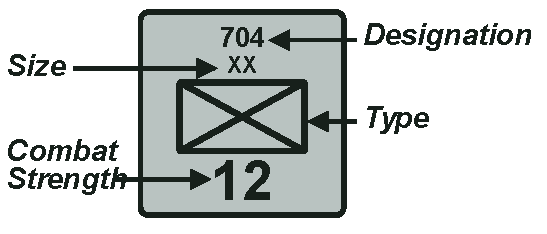
\includegraphics[width=\linewidth]{figures/counter-anatomy.pdf} &
  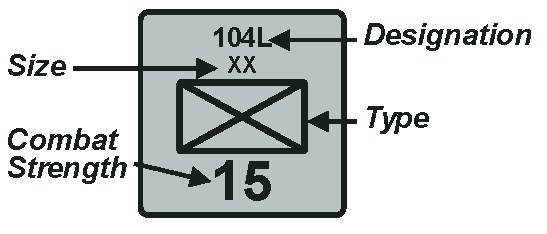
\includegraphics[width=\linewidth]{figures/counter-anatomy-german-back.pdf} \\
  \scriptsize Front & \scriptsize Back
\end{tabular}
\end{center}

{\sffamily\bfseries Guerrilla Group (Partisan)\par}
\vspace{2pt}
\begin{center}
\begin{tabular}{@{}>{\centering\arraybackslash}m{0.46\linewidth}@{\hspace{0.02\linewidth}}>{\centering\arraybackslash}m{0.46\linewidth}@{}}
  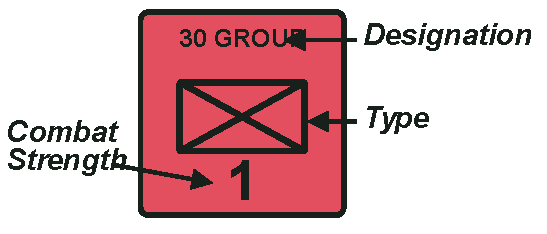
\includegraphics[width=\linewidth]{figures/counter-anatomy-partisan-front.pdf} &
  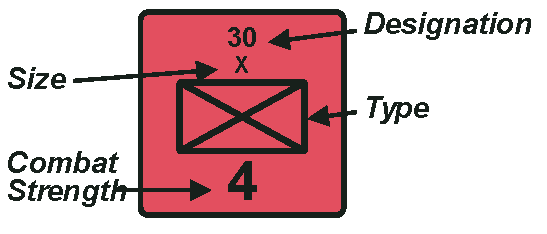
\includegraphics[width=\linewidth]{figures/counter-anatomy-partisan-back.pdf} \\
  \scriptsize Front & \scriptsize Back
\end{tabular}
\end{center}

Guerrilla groups possess no unit-size symbol; their reverse side may represent
a different organizational size.

\needspace{15\baselineskip}
\case{2.23} \textbf{Summary of Unit Types}

\begin{center}
{\sffamily\bfseries Combat\par}
\vspace{3pt}
\begin{tabular}{@{}c c c c@{}}
  \counterimage[0.17\linewidth]{italian-infantry} &
  \counterimage[0.17\linewidth]{partisan-infantry} &
  \counterimage[0.17\linewidth]{german-mechanized-infantry} &
  \counterimage[0.17\linewidth]{german-mountain-infantry} \\
  \scriptsize \shortstack{Infantry\\(Italian)} &
  \scriptsize \shortstack{Infantry\\(Partisan)} &
  \scriptsize \shortstack{Mechanized\\Infantry} &
  \scriptsize \shortstack{Mountain\\Infantry} \\
  \addlinespace[4pt]
  \counterimage[0.17\linewidth]{german-panzer} &
  \counterimage[0.17\linewidth]{german-cavalry} &
  \counterimage[0.17\linewidth]{german-parachute} &
  \counterimage[0.17\linewidth]{tito-unidentified} \\
  \scriptsize Panzer & \scriptsize Cavalry & \scriptsize Parachute & \scriptsize Tito \\
  \addlinespace[4pt]
  \counterimage[0.17\linewidth]{tito-identified} &
  \counterimage[0.17\linewidth]{partisan-group} &
  \counterimage[0.17\linewidth]{partisan-brigade} & {} \\
  \scriptsize \shortstack{Tito\\identified} &
  \scriptsize \shortstack{Partisan\\group} &
  \scriptsize \shortstack{Partisan\\brigade} & {}
\end{tabular}

\medskip
{\sffamily\bfseries Markers\par}
\vspace{3pt}
\begin{tabular}{@{}c c c c@{}}
  \counterimage[0.17\linewidth]{victory-points} &
  \counterimage[0.17\linewidth]{allied-progress} &
  \counterimage[0.17\linewidth]{game-turn} &
  \counterimage[0.17\linewidth]{drought-turn} \\
  \scriptsize \shortstack{Victory\\Points} &
  \scriptsize \shortstack{Allied\\Progress} &
  \scriptsize \shortstack{Game\\Turn} &
  \scriptsize \shortstack{Drought\\Turn}
\end{tabular}
\end{center}

\textbf{Nationality colors}

\begin{center}
\begin{tabular}{@{}c c c c@{}}
  \counterimage[0.17\linewidth]{german-infantry-front} &
  \counterimage[0.17\linewidth]{serbian-infantry} &
  \counterimage[0.17\linewidth]{italian-infantry} &
  \counterimage[0.17\linewidth]{croat-infantry} \\
  \scriptsize German & \scriptsize Serbian & \scriptsize Italian & \scriptsize Croat \\
  \addlinespace[4pt]
  \counterimage[0.17\linewidth]{bulgarian-infantry} &
  \counterimage[0.17\linewidth]{soviet-infantry} &
  \counterimage[0.17\linewidth]{partisan-group} &
  \counterimage[0.17\linewidth]{chetnik-group} \\
  \scriptsize Bulgarian & \scriptsize Soviet & \scriptsize Partisan & \scriptsize Chetnik
\end{tabular}
\end{center}

The front and reverse side of certain units are sometimes employed for entirely
different purposes in terms of the game.

\case{2.24} \textbf{Unit Size Symbols.} A unit's size plays an important role in
the game: II = Battalion; III = Regiment; X = Brigade; XX = Division; and XXX =
Corps. Guerrilla groups possess no size symbol.

\subsection{Parts Inventory}\label{sec:2.3}

\begin{itemize}
  \item one 22-by-34-inch map;
  \item one 200-counter die-cut counter sheet;
  \item one 12-page rules booklet;
  \item one six-sided die (not included in the \emph{S\&T} edition); and
  \item one game-box assembly (not included in the \emph{S\&T} edition).
\end{itemize}

\begin{historicalnote}
The original booklet directed owners to SPI's Rules Questions Editor and
Complaint Card for replacement parts and rules questions. Those services and
the printed New York mailing address are preserved in the source scan but are
no longer active.
\end{historicalnote}
